% !TeX root=main.tex

\section{Methodik der Thesis}

Die Methodik dieser Bachelorthesis basiert auf einer Kombination aus einer Literaturrecherche und Expertenbefragung. Diese Methodenkombination ermöglicht es, ein fundiertes theoretisches Fundament zu legen und gleichzeitig praktische Einblicke zu gewinnen, um die Forschungsfragen zu beantworten.

\begin{figure}[H]
    \centering
    \caption{Aufbau und Struktur der Bachelorthesis mit Forschungsmethodik}
    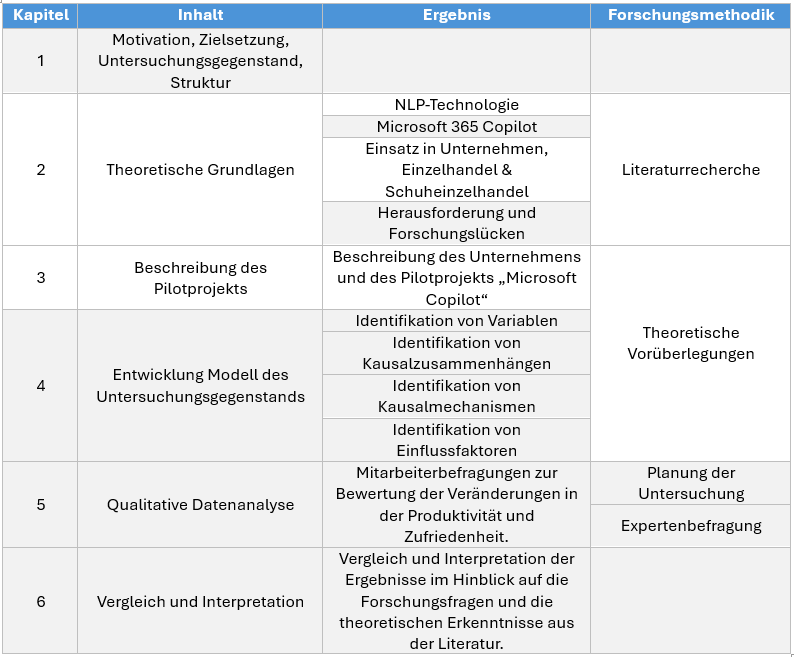
\includegraphics[scale=0.7]{methodik}
    \captionsetup{font=scriptsize}
    \label{fig:methodik}
\end{figure}

Die Methodik theoretischen Vorüberlegungen und der Expertenbefragung basiert auf bewährten Ansätzen von Gläser und Laudel\footnote{Vgl. \cite{Glaeser2010}}. Gläser und Laudel beschreiben die Forschungsmethodik als einen systematischen Prozess, um wissenschaftliche Fragestellungen zu beantworten. Die Methodik besteht aus einer strukturierten Vorgehensweise, um die Forschungsfragen zu beantworten und die Relevanz der Ergebnisse zu evaluieren. Die Methodik besteht aus folgenden Schritten: 
\begin{itemize}
    \item die Formulierung der Untersuchungsfrage, die mit einer Wahl einer Erklärungsstrategie verknüpft ist
    \item die theoretische Vorüberlegung
    \item die Planung der Untersuchung
    \item Erhebungs- und Auswertungsmethoden
\end{itemize}

Die Methodik der Literaturrecherche basiert auf dem Ansatz vom Brocke et al. \footnote{Vgl. \cite{Brocke2009}, S. 205-224}
und wurde bereits begonnen. Die Literaturrecherche wurde auf folgenden Plattformen durchgeführt:

\begin{itemize}
    \item BASE: \underline{\textcolor{blue}{https://www.base-search.net/}}
    \item Web of Science: \underline{\textcolor{blue}{https://www.webofscience.com/wos/}}
\end{itemize}

Bei der Literaturrecherche gibt es zwei zentrale Herausforderungen. Erstens gilt es, das relevante Wissen zum Thema zu identifizieren. Zweitens muss unterschieden werden, welches Wissen relevant und welches irrelevant ist. Um diese Herausforderungen zu bewältigen, orientiere ich mich an den Empfehlungen von Fragen von Gläser und Laudel\footnote{Vgl. \cite{Glaeser2010}, S.76}, die Unterstützung bei der Recherche bieten:

\begin{enumerate}
    \item Gibt es Theorien, die das Untersuchungsobjekt (empirische Feld) als Thema behandeln? Welche Theorien lassen sich auf das Untersuchungsobjekt anwenden, wenn allgemeine Begriffe für das empirische Feld verwendet werden? Wurden einzelne Aspekte der gleichen Disziplin in anderen Arbeiten bereits erforscht?
    \item Gibt es Theorien, die aufgrund von Eigenschaften des Untersuchungsobjekts ausgeschlossen werden können? Beinhalten die Theorien Voraussetzungen, die in meinem Untersuchungsfeld nicht anwendbar sind?
\end{enumerate}

Das empirische Feld meiner Untersuchung ist der Einsatz von KI-basierten Tools, insbesondere Microsoft 365 Copilot, in Unternehmen, mit besonderem Fokus auf den Schuheinzelhandel. Diese Untersuchung ist in der Disziplin der Wirtschaftsinformatik oder der Technologiemanagements mit Überschneidungen zur Betriebswirtschaftslehre und Organisationspsychologie. Die allgemeinen Begriffe meines empirischen Felds lassen sich mit Digitale Transformation, Künstliche Intelligenz im Unternehmenskontext, Prozessoptimierung, Arbeitsplatzautomatisierung und Technologieadoption in Unternehmen beschreiben. Die Spezifika des empirischen Felds sind der Fokus auf NLP- Tools, Spezifische Anwendung im Schuh-/ Einzelhandel, Betrachtung der Auswirkung auf Effizienz und Produktivität und Einbeziehung von Microsoft 365 Copilot als konkretes Beispiel. Durch die Spezifika des Untersuchungsobjekt können nach erstem Überblick der Stand der Forschung die allgemeinen Theorien mit dem Fokus auf Industrieautomatisierung und KI-Technologien, die nicht NLP-Tools sind, wie bspw. Deep Learning, von dem weiteren Literaturstudium ausgeschlossen werden. 
Aus den Merkmalen und Spezifikationen habe ich folgende Suchabfrage entwickelt:
\begin{verbatim}
("natural language processing" OR "NLP" OR "Microsoft 365 Copilot") 
AND 
("business process*" OR "work process*" OR "workflow*" 
    OR "digital transformation" OR "technology adoption") 
AND 
("retail" OR "shoe retail*" OR "footwear industry" OR "commerce" 
    OR "business" OR "enterprise*" OR "company" OR "companies") 
AND 
("efficiency" OR "productivity") 
\end{verbatim}

Zunächst wurde die Suchanfrage in der Datenbank BASE in allen Feldern durchgeführt, was zu 252 Treffern führte. Anschließend wurde die Suche auf Schlagwörter eingegrenzt, wodurch 87 Treffer erzielt wurden. Im weiteren Verlauf wurden nur die Quellen berücksichtigt, die öffentlich und kostenlos zugänglich waren. Somit wurde eine Anzahl von 44 empirische Artikel, auf denen der empirische Fokus lag, erreicht. Zuletzt wurden eine manuelle Selektion von irrelevanten Quellen, wie bspw. aus der Medizin, für diese Arbeit, mithilfe von den Informationen aus dem Abstract durchgeführt, sodass eine Literaturanzahl von 17 Treffern aus der Literaturdatenbank BASE erreicht wurde.

Um nicht nur eine Quelle für die Literatursuche verwendet wurde, wurde zudem die Datenbank Web of Science als zweite Datenbank für eine weitere suche von Literatur herangezogen. Dabei wurde die gleiche Suchabfrage, wie auch in der Abfrage in der Datenbank BASE, verwendet. Bei der Abfrage wurden 66 Ergebnisse gefunden, die weiter eingegrenzt wurden mit dem „Research Area“ Filter auf „Computer Science“, um die Ergebnisse auf 53 Treffer zu erreichen. Für eine weitere Beschränkung wurde der „Document Types“ Filter auf „Article“ gesetzt (n=32). Des Weiteren wurden die Abstracts durchgelesen, um die Literatur manuell zu den relevanten Inhalten zu filtern. Dabei wurden die Inhalte, die sich sehr auf die technischen Hintergründe von NLP fokussieren oder sich zu sehr auf Geschäftsprozessmodellierung konzentrieren, von der weiteren Literaturrecherche ausgeschlossen. Ausgeschlossen von der weiteren Suche wurden auch die Literatur, die sich auf die Fertigungsindustrien oder Medizin fokussierten. Somit wurde eine Trefferanzahl von 12 Literaturquellen aus der Datenbank Web of Science erreicht.

\begin{figure}[H]
    \centering
    \caption{Datenbankrecherche}
    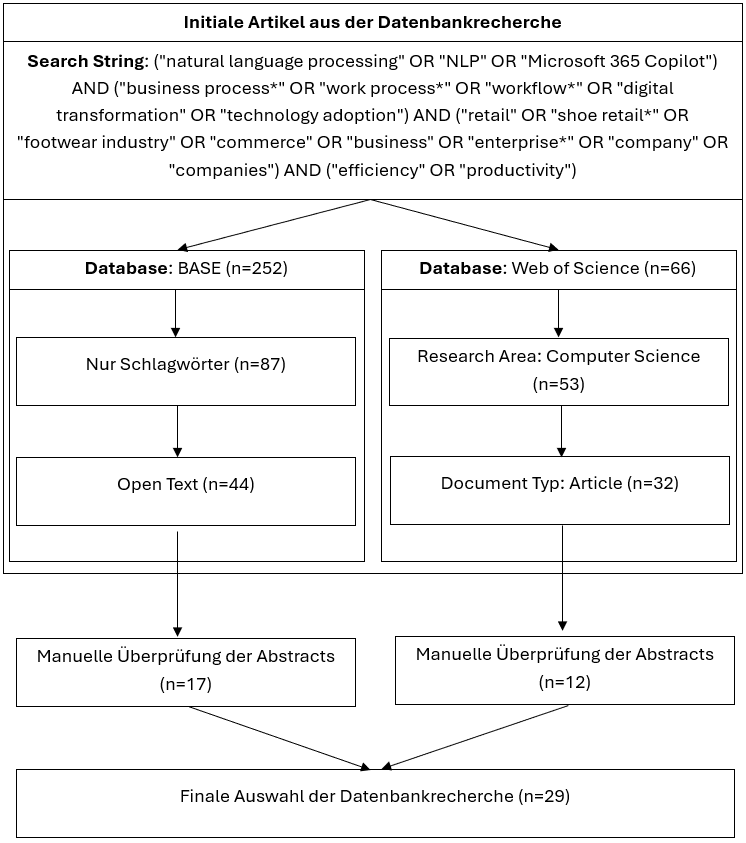
\includegraphics[scale=0.7]{datenbankrecherche}
    \captionsetup{font=scriptsize}
    \label{fig:methodik}
\end{figure}

Bei der Datenbankrecherche wurden zahlreiche Referenzen zu Themen wie den aktuellen Herausforderungen der NLP-Integration in Arbeitsprozesse, der Zusammenarbeit zwischen Menschen und KI, dem Einsatz von NLP in Unternehmen sowie der digitalen Transformation und der Erläuterung der NLP-Technologie gefunden. Auch zur Positionierung und zu Forschungsfragen für die Arbeit sind Informationen vorhanden. Allerdings zeigte die Datenbankrecherche weniger Erfolg bei der Beschaffung von Informationen zu den Themen NLP und Soziales, Definitionen und Modelle der Produktivität und Effizienz, Microsoft 365 Copilot sowie dem Einsatz von NLP im Einzelhandel oder speziell im Schuheinzelhandel.

Aufgrund der fehlenden Informationen zu den genannten Themenbereichen wird die Literaturrecherche erweitert mit dem KI-Tool Elicit (\underline{\textcolor{blue}{https://elicit.com/}}). Elicit  verfügt über trainierte Sprachmodelle, die relevante Forschungsartikel anhand von Fragen oder Stichworten finden. Das Sprachmodell generiert Zusammenfassungen jedes Forschungsartikels. Fast 2 Millionen Menschen nutzen dieses Tool für verschiedene Zwecke. Forscher bei Google, Stanford, der NASA und der Weltbank nutzen Elicit, um ihren Forschungsprozess zu beschleunigen. Es enthält fast 125 Millionen wissenschaftliche Arbeiten aus dem Semantic Scholar-Korpus, der alle akademischen Disziplinen abdeckt.\footnote{Vgl. \cite{EduTools2024}}

\begin{longtable}{|p{9cm}|p{3cm}|}
    \caption{Ergebnisse der Elicit-Suche} \label{tab:elicitergebnisse} \\
    \hline
    \textbf{Prompt} & \textbf{Trefferanzahl} \\
    \hline
    How does the use of AI-based tools such as Microsoft 365 Copilot influence the efficiency and productivity of administrative work processes in companies? & n=6 \\
    \hline
\end{longtable}

\clearpage